\section{The Ambition That Ate The Marriage}

\subsection{Selling the Soul He Thought He Was Saving}

``You said no more of this,'' Emma said from the doorway while flipping the hallway switch with a snap. The overhead light 
washed the room in white.

The kitchen had the polished chill of a showroom: quartz counters, brushed steel appliances, a reclaimed wood island 
that still smelled faintly of lemon oil and garlic. The dinner dishes were stacked in the sink, mostly untouched. 
A half-empty bottle of scotch stood like a forgotten prop near the fruit bowl. Above the stove, a digital clock 
glowed 2:11 a.m.

Outside, a thin sheet of snow drifted against the glass door leading to the backyard, where the swing set sat unused. 
Inside, the room was still — not quiet, exactly, but paused, like a breath being held.

David didn’t look up. ``It’s just one last push.''

She looked at him sternly. ``You said that last week. And the week before.'' 

She said this while fighting to keep her voice steady.

He lifted his eyes to meet her gaze. ``This one’s different. I’m speaking tomorrow. The conference panel—''

``—doesn’t tuck the kids in,'' she cut in.

His eyes shifted briefly toward the fridge. Taped near the handle was a photo of the kids in Halloween costumes: a picachu 
and a care bear. One of them had drawn crooked lightning bolts around the border with a blue marker. He stared at it for a 
moment too long.

She doesn’t understand, he thought. Not really. Not what it means to carry the weight of something invisible. Not what it’s 
like to wake up with ambition burning holes in your gut and go to bed still feeling behind. This wasn’t about ego. It was 
about survival. It was about legacy. It was about keeping them safe in a world that didn’t care.

He sat at the island, still in his t-shirt from the day before. The light from his laptop screen cast pale-blue shadows 
across the counter. Slide 14 was on the screen again: \textit{Risk Stratification Under Uncertainty}. He adjusted a 
y-axis, then stared at it like it owed him something.

Emma walked to the fridge, opened it, and just stood there, unmoving. A bottle of wine shifted slightly but she let it 
settle. The soft whir of the appliance filled the silence between them.

``You promised this would be better,'' she said. ``That starting your own business meant more time for us. Not... 
whatever this is.''

He sighed. ``You know this is for us, right? The whole point is—''

``You’re pitching to your wife at two in the morning. Do you hear yourself?'' she cut in again but this time in a cold voice.

He turned. ``I’m trying to build something that lasts.''

Emma leaned on the counter with her arms crossed. ``What if we already have something that lasts, and you’re too busy optimizing 
it into oblivion?''

He didn’t answer. She glanced at the screen.  ``Let me guess. Twenty-five slides, and zero about what it’s costing you.''

``It’s costing us now so it doesn’t later.'' 

When David said it he wasn't quite sure if he was telling his wife it or himself. 

She looked at him the way someone looks at a person they love when they suspect the real goodbye already 
happened months ago.

``Just... don’t sell your soul.'' she said in a resigned voice.

David smiled, the kind of smile that knew too much and said too little. ``I would never do that. I’m doing this for us.''

She didn’t argue. That was the part that landed harder.

``That’s what makes it scarier,'' she said, and walked away.

The sound of her slippers faded down the hall, muffled but final. The house seemed colder without her in the room. 
David sat there, unmoving.

Then, quietly, he deleted the phrase ``adaptive resilience'' and typed:

\textbf{Compliant AI Infrastructure for Enterprise Risk.}

He stared at it.

Then clicked save.


\medskip

\begin{PsychologicalSidebar}{The Builder’s Paradox}

  David isn’t selfish. He’s committed.

  \medskip
  
  That’s what makes it dangerous.
  
  \medskip
  
  In Cognitive Behavioral Therapy (CBT), there’s a class of mental traps called \textbf{cognitive distortions}: 
  patterns of thought that feel rational, but quietly sabotage well-being.

  \medskip
  
  David’s internal script checks multiple boxes:

  \medskip
  
  \begin{itemize}
    \item \textbf{All-or-Nothing Thinking:} “If I don’t make this work, I’ve failed my family.”
    \item \textbf{Fortune Telling:} “Once this deal closes, things will calm down.”
    \item \textbf{Emotional Reasoning:} “I feel guilty when I rest; therefore, I must not deserve to rest.”
  \end{itemize}
  
  \medskip
  
  These distortions feed into a larger psychological dynamic:  
  \textbf{goal substitution}. This happens when a person replaces a real goal (family, connection, presence) 
  with a symbolic one (success, income, prestige) because the latter is easier to measure and harder to challenge.

  \medskip
  
  Over time, the means becomes the mission.  
  The system becomes self-justifying.  
  And the more sacrifice he makes, the more he feels obligated to make it worth something: a classic \textbf{sunk cost fallacy}.
  
  \medskip
  
  That’s why Emma’s words don’t break through.  
  David’s not ignoring her. He’s defending a narrative that keeps him going.
  
  \medskip
  
  So when he hits “save,” he’s not just preserving a PowerPoint.
  He’s reaffirming a distortion.  
  And crossing a line he doesn’t fully see... yet.
  
\end{PsychologicalSidebar}

\subsection*{Editor Questions for ``Selling the Soul He Thought He Was Saving''}

To get meaningful and diverse feedback, I designed these questions to go beyond surface-level edits. 
I need you to reflect not just on technical clarity or style, but on emotional resonance, character 
believability, narrative structure, pacing, and thematic depth. You don’t need to answer every question. 
Please focus on the ones that speak to your experience as a reader. The goal is not to fix the scene, but 
to understand how it lands, where it connects, and where it might quietly miss.


\subsubsection{Narrative \& Structure}

\begin{itemize}
  \item Did this feel like the right way to open the story? Why or why not?
  \item Was the pacing effective? Did it hold your attention throughout the scene?
  \item Did anything feel redundant or like it could be trimmed without losing impact?
\end{itemize}

\subsubsection{Emotional Resonance}

\begin{itemize}
  \item How did this scene make you feel? Were you more aligned with David, Emma, or torn?
  \item Did Emma’s final line (“That’s what makes it scarier”) land for you emotionally? Why or why not?
  \item Was there a moment where you really felt the tension — or where it broke?
\end{itemize}

\subsubsection{Character Insight}

\begin{itemize}
  \item Did David feel like a real person to you? Did his motivations make sense?
  \item Did Emma’s dialogue and reactions feel grounded and believable?
  \item What assumptions do you find yourself making about their relationship based on this scene?
\end{itemize}

\subsubsection{Psychological Sidebar}

\begin{itemize}
  \item Did the psychological sidebar enhance your understanding of David? Or did it feel like too much explanation?
  \item Would you prefer the sidebar be integrated into the narrative or kept separate like this?
  \item Was anything in the sidebar particularly insightful or redundant?
\end{itemize}

\subsubsection{Theme \& Message}

\begin{itemize}
  \item What do you think this scene is ultimately about?
  \item Did it raise any personal or philosophical questions for you?
  \item Do you feel like this is “just a marriage scene,” or something larger about ambition, modern work, or identity?
\end{itemize}

\subsubsection{Style \& Craft}

\begin{itemize}
  \item Was there a line or image that stuck with you — positively or negatively?
  \item Did the rhythm of the dialogue feel natural?
  \item Did you notice any clichés or overused tropes that undercut the scene’s originality?
\end{itemize}

\subsubsection{Deeper Testing}

\begin{itemize}
  \item How would your impression of David change if the sidebar wasn’t included?
  \item If you had to cut 20\% of this section, what would go?
  \item If you read this cold — with no context — what genre or tone would you expect the rest of the story to take?
\end{itemize}

\subsection{The Morning After}

David never went to sleep.

He had stared at the screen until the slide blurred, the typeface swimming in his peripheral vision 
like noise underwater. By 5:42 a.m., he was editing bullet points more out of inertia than purpose. 
The house was still dark except for the glow of the monitor and the amber halo of the hallway nightlight.

Then he heard the soft patter of bare feet on the hardwood.

It was Oliver, the youngest. Hair tousled, clutching a stuffed octopus by the neck.

``Daddy?''

David turned in his chair. ``Hey, buddy.''

The boy rubbed his eyes, blinked, and asked the question with a seriousness that never failed to break 
David’s heart: ``Are you leaving again?''

David smiled, knelt down, and pulled him into a hug. ``Not yet.''

Ten minutes later, both kids were in the kitchen. David, still in yesterday’s shirt, last night’s mind, and now 
rummaged through cabinets. He found pancake mix, a nonstick pan, and the chipped blue bowl that Emma never 
threw out because it reminded her of their first apartment. He stirred batter like he had muscle memory 
for it, flipping pancakes while refereeing an argument about syrup ratios.

By the time the second batch was browning, the noise must’ve reached upstairs. Emma walked into the kitchen 
wearing a loose sweater and a sleep-creased face while blinking at the brightness and the smell of butter and maple.

She paused.

``You’re... making breakfast?''

He looked over his shoulder. ``Emergency chef coverage. The regular guy called out.''

Emma chuckled softly and took a seat at the island, where the kids were already giggling over a lopsided 
pancake that looked vaguely like Pikachu.

They ate together, the four of them, at the kitchen counter. No rush. No schedules. Just shared space. Shared 
syrup. Shared warmth.

And for a brief, flickering moment, it felt like something whole.

David kept sneaking glances at Emma. She smiled more in that one hour than he could remember in weeks. Not the 
polite smile she wore at client dinners or the tight-lipped nod she gave when he said he was ``almost done.''
A real smile. Soft around the eyes. Present.

He tried to lock it into memory.

He couldn’t remember the last time she had actually enjoyed his company. Not tolerated it. Not supported it. 
Enjoyed it.

Since the kids came, their connection had been rerouted. She had grown closer to them in ways that felt 
untouchable. Protective. Intimate. Complete. And David had grown further from her, not out of malice, 
but out of momentum.

He didn’t blame her. She had every right to turn toward the people who needed her back.

And he? He told himself he would make it up to her. He would make it up to all of them.
The late nights. The missed recitals. The silent gaps in the marriage.

He would make it all worth it.

Someday.

Because this wasn’t about escape. It was about building something they could all live inside.
Something resilient. Something strong.

Even if it meant he had to stand outside of it for a while.

After breakfast, he kissed them all --- quick, like punctuation --- and grabbed his bag by the door.

His flight was in two hours.

But all he could think about was the warmth of syrup on her fingers.
And the way she smiled when she thought he wasn’t looking.


\subsection*{Editor Questions for ``The Morning After''}

This scene is quieter — more atmospheric than expository. The goal of these questions is to help surface what’s working on a subtle, emotional level and where it might land softer than intended. Focus on the resonance, intimacy, and implied stakes. You don’t have to answer everything — just respond where you felt something shift.

\subsubsection{Narrative \& Structure}

\begin{itemize}
  \item Did the scene unfold at the right pace for its tone? Was anything rushed or overly drawn out?
  \item How well did the transition from solitude to domestic warmth land for you as a reader?
  \item Was there a moment that felt like the emotional or narrative pivot? Did it arrive at the right time?
\end{itemize}

\subsubsection{Emotional Resonance}

\begin{itemize}
  \item What did this scene make you feel — and when did you feel it most?
  \item Did David’s emotional undercurrent (guilt, longing, resolve) come through clearly?
  \item Did the warmth of the scene feel earned, or did it risk sentimentality?
\end{itemize}

\subsubsection{Character Insight}

\begin{itemize}
  \item Did David’s actions (making breakfast, watching Emma) feel honest to who he is?
  \item What do you learn about Emma, even though she says very little?
  \item What does this scene suggest about the emotional architecture of their marriage?
\end{itemize}

\subsubsection{Scene Texture}

\begin{itemize}
  \item Did the domestic details (pancakes, syrup arguments, chipped bowl) enhance your immersion?
  \item Was there a moment that felt especially visual or sensory for you?
  \item Did the contrast between David’s professional world and this kitchen scene feel intentional — or like a temporary escape?
\end{itemize}

\subsubsection{Theme \& Message}

\begin{itemize}
  \item What do you think this scene is ultimately about: redemption, guilt, sacrifice, or something else?
  \item Did the “someday” refrain (about making it up to them) feel hollow, hopeful, or heartbreaking?
  \item Did this scene add depth to your understanding of David’s internal conflict? If so, how?
\end{itemize}

\subsubsection{Style \& Craft}

\begin{itemize}
  \item Was there a line or gesture that lingered with you after reading?
  \item Did the rhythm of the prose mirror the emotional tone?
  \item Did anything feel overwritten or unnecessary given the softness of the moment?
\end{itemize}

\subsubsection{Deeper Testing}

\begin{itemize}
  \item What would change emotionally if this scene were cut from the story?
  \item If the scene ended just before the breakfast — or just after the flight — would it be stronger or weaker?
  \item If you were reading this as part of a longer work, what expectations would this scene set for what’s to come?
\end{itemize}











\subsection{The Ride to the Airport}

The Uber was a black Escalade with cooled leather seats and the faint smell of eucalyptus from a vent 
clip in the dash. David climbed in, offered a nod to the driver, and settled into the backseat. The 
city outside was still shaking off the morning: joggers with earbuds, cafes flipping signs, and garbage 
trucks doing their work like it mattered.

David opened his laptop.

Slide 14 greeted him again, unchanged from the night before:
\textit{Risk Stratification Under Uncertainty.}

But now he had to move faster.

He wasn’t behind because of laziness. He was behind because of pancakes. Because of syrup. 
Because his son had asked if he could stay just five more minutes... and he had.

So here he was, revising in transit, because he chose to make breakfast.

And even with the mounting pressure, he didn’t regret it.

He clicked through his deck with the methodical pace of a surgeon reviewing x-rays. Slide by slide, the story emerged
about how his startup could automate the soul-crushing grind of regulatory compliance.

Not just dashboards or alerts.

\textit{Narrative automation. Report generation. Fully auditable traceability.}

Because financial institutions were required to submit mountains of documentation to regulators, and while the 
rules varied slightly across jurisdictions — Basel, Dodd-Frank, ESMA, MAS — the structural bones were always the same:
\textbf{classify, justify, certify}.

\medskip

\begin{HistoricalSidebar}{A Brief History of Financial Regulation Reporting}

    Modern financial reporting requirements are the aftershocks of crisis.
    
    \medskip
    
    After the 1929 stock market crash, the U.S. passed the \textbf{Securities Act of 1933} and the 
    \textbf{Securities Exchange Act of 1934}, giving rise to the SEC and enshrining the principle 
    of disclosure: \textit{you don’t have to be honest, but you do have to report what you’re doing 
    so someone can check}. Annual 10-Ks, quarterly 10-Qs, and a cascade of schedules followed.
    
    \medskip
    
    In the decades that followed, regulation often lagged innovation. Derivatives exploded in the '80s. 
    Risk reporting didn’t catch up until the \textbf{Basel Accords}, a series of international banking 
    standards set by the Basel Committee beginning in 1988. Basel I introduced capital requirements. 
    Basel II added “risk-weighted assets.” Basel III came after the 2008 financial crisis and emphasized 
    stress testing, liquidity coverage, and leverage ratios. Each step added layers of required documentation 
    — and interpretive gray zones.
    
    \medskip
    
    Meanwhile, the U.S. Dodd-Frank Act of 2010, passed in the wake of the global financial crisis, created 
    more than 400 new rules and mandated detailed documentation of systemic risk, trading activity, third-party 
    exposure, and internal controls. Institutions had to file Form PFs, living wills, swap data reports, and 
    CCAR submissions. Europe responded with its own: \textbf{MiFID II}, \textbf{EMIR}, \textbf{CRD IV}.
    
    \medskip
    
    But no matter the jurisdiction, the workflow was the same:

    \medskip

    \begin{enumerate}
    \item \textbf{Classify} the assets and exposures.
    \item \textbf{Justify} the risk methodologies and controls.
    \item \textbf{Certify} compliance through formal attestation and documentation.
    \end{enumerate}
    
    \medskip
    
    Regulators didn’t demand certainty — they demanded \textit{coherence}. And that meant narrative. Every 
    number had to be explained. Every position had to be defended.
    
    \medskip
    
    By the 2020s, the volume of regulatory reporting had grown so massive that it quietly spawned an entire 
    cottage industry — RegTech — with startups offering software to automate filings, format disclosures, and 
    validate transaction records.
    
    \medskip
    
    But David’s insight went a step further:
    \textbf{What if the reports didn’t just comply with regulation? What if they interpreted it too?}

    \medskip
    
    Because the regulators weren’t just asking for answers.
    They were asking if you understood the question.

\end{HistoricalSidebar}

\medskip

The regulation, David liked to say, wasn’t math. It was scripture.
And scripture is interpreted.

But ninety percent of it wasn’t even interpretation. It was repetition.
Same tables. Same language. Same formatting.
Most risk officers were glorified stenographers who copy structured data from one box into another.
However, that's not the hard part. The hard part is making sense of the data.

So David's solution was simple:
\textbf{train a model to interpret the scriptures faster than the priests.}

His slides detailed the pipeline.

\medskip

\begin{figure}[H]
    \centering
    \resizebox{0.85\textwidth}{!}{%
      \begin{tikzpicture}[
        font=\footnotesize,
        stage/.style={draw=black, thick, rounded corners, minimum width=3.6cm, minimum height=1.6cm, align=center, fill=gray!10},
        arrow/.style={->, thick},
        node distance=1.5cm and 2.6cm
      ]
  
      % Top Row (left to right)
      \node[stage] (extract) at (0,0) {
        \parbox{3.4cm}{
            \centering \textbf{Extract} \\\ \\
            \begin{itemize}
                \item Transaction logs 
                \item Margin calls
            \end{itemize}
          }
      };
  
      \node[stage, right=of extract] (model) {
        \parbox{3.4cm}{
            \centering \textbf{Interpret} \\\ \\
            \begin{itemize}
                \item Risk heuristics
                \item Data context
            \end{itemize}
        }
      };
  
      % Downward arrow to next tier
      \node[stage, below=2.2cm of model] (generate) {
        \parbox{3.4cm}{
            \centering \textbf{Generate Narrative} \\\ \\
            \begin{itemize}
                \item Summaries 
                \item Analysis
            \end{itemize}
        }
      };
  
      \node[stage, left=of generate] (deliver) {
        \parbox{3.4cm}{
            \centering \textbf{Deliver} \\\ \\ 
            \begin{itemize}
                \item PDFs 
                \item Audit trails
            \end{itemize}
        }
      };
  
      % Arrows
      \draw[arrow] (extract) -- (model);
      \draw[arrow] (model) -- ++(0,-1.2) -- (generate.north);
      \draw[arrow] (generate) -- (deliver);
  
      \end{tikzpicture}%
    }
    \caption{Slide Snapshot: Snake-style pipeline from data extraction to regulatory narrative delivery.}
\end{figure}

\medskip

Most RegTech startups solved for formatting.

They offered tools that ingested data, standardized it across jurisdictions, and outputted XML or JSON 
in regulator-approved schemas. They built dashboards that tracked deadlines, flagged anomalies, and 
generated templated disclosures based on pre-defined rules.

But their systems were reactive.

They followed the letter of compliance, and not its spirit. They automated checklists, not judgment. Their 
``AI'' was often just glorified decision trees hidden behind polished UIs.

\medskip

\begin{figure}[H]
    \centering
    \resizebox{0.85\textwidth}{!}{%
      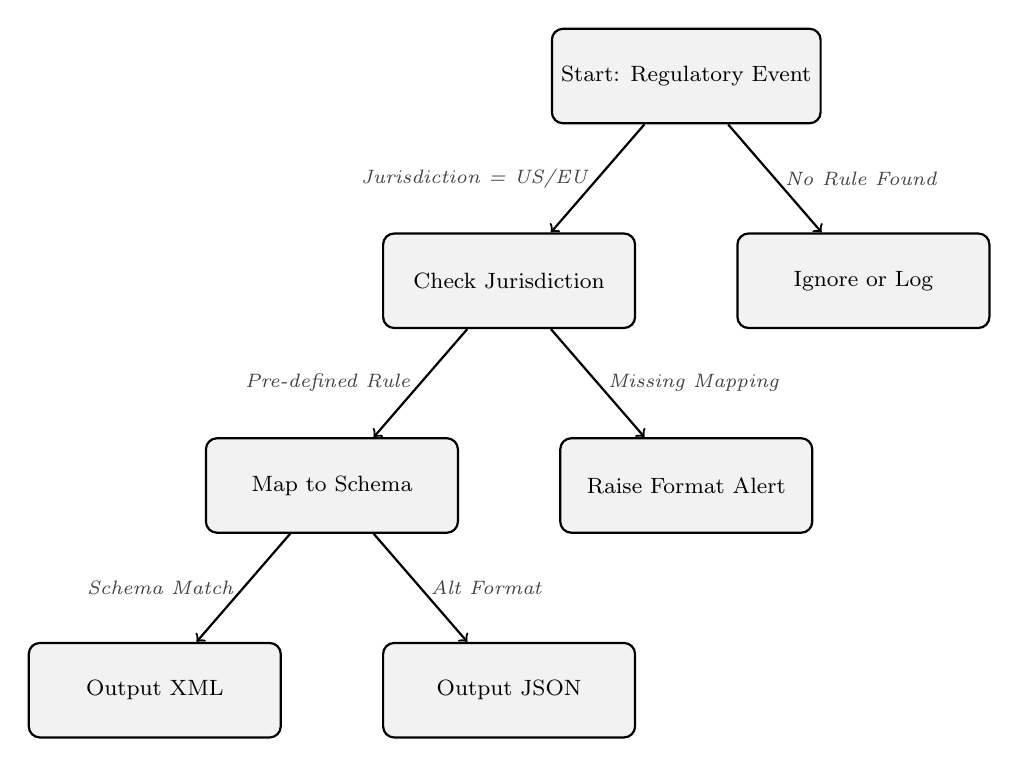
\begin{tikzpicture}[
        font=\footnotesize,
        node/.style={draw, rounded corners, align=center, minimum width=3.2cm, minimum height=1.2cm, fill=gray!10, thick},
        edge from parent/.style={draw, thick, ->},
        level distance=2.6cm,
        sibling distance=4.5cm,
        metadata/.style={font=\scriptsize\itshape, text=gray!50!black}
      ]
  
      \node[node] {Start: Regulatory Event}
        child { node[node] {Check Jurisdiction}
          child { node[node] {Map to Schema}
            child { node[node] {Output XML} 
              edge from parent node[midway, left, metadata] {Schema Match} }
            child { node[node] {Output JSON}
              edge from parent node[midway, right, metadata] {Alt Format} }
            edge from parent node[midway, left, metadata] {Pre-defined Rule}
          }
          child { node[node] {Raise Format Alert}
            edge from parent node[midway, right, metadata] {Missing Mapping}
          }
          edge from parent node[midway, left, metadata] {Jurisdiction = US/EU}
        }
        child { node[node] {Ignore or Log}
          edge from parent node[midway, right, metadata] {No Rule Found}
        };
  
      \end{tikzpicture}%
    }
    \caption{Illustrative Decision Tree: A simplified RegTech compliance system built on pre-defined rules and 
    deterministic formatting logic.}
\end{figure}

\medskip

David’s pipeline was different.

It wasn’t just built to file forms. It was built to reason.
Where startups parsed static fields, David’s models digested narrative.
Where others validated with if-statements, he mimicked analyst intuition.
Where others summarized in bullets, he wrote paragraphs in the voice of a junior compliance officer.
And most critically, where others stopped at formatting, he captured \textit{justification}.

Because he understood what most vendors didn’t.
\textbf{Regulators don’t want answers. They want accountability in prose.}

\medskip

\begin{HistoricalSidebar}{Scripture, Commentary, and the Politics of Interpretation}

    Religious texts are not read. They are interpreted.
    And interpretation, throughout history, has been the real seat of power.
    
    \medskip
    
    The \textbf{Qur’an}, for instance, is considered by Muslims to be the literal word of God. But its 
    application in everyday life is shaped not just by the Qur’an itself, but by the \textbf{Hadiths} --- 
    collections of sayings and actions of the Prophet Muhammad --- and by generations of \textbf{tafsir} 
    (interpretive commentary) authored by scholars, jurists, and theologians.
    
    \medskip
    
    Similarly, the \textbf{Torah} — the foundational text of Judaism — is accompanied by layers of 
    interpretive tradition, including the \textbf{Mishnah}, \textbf{Talmud}, and countless rabbinical commentaries. 
    Jewish legal rulings (halakha) don’t come directly from the Torah, but from how generations of rabbis 
    debated and interpreted its words.
    
    \medskip
    
    Even the Protestant Reformation wasn’t a dispute over which Bible to read. It was a dispute over how to 
    interpret it. \textbf{Luther} and \textbf{Calvin} read the same scriptures. But their commentaries ---
    their theological models --- diverged in ways that reshaped Europe.  

    \medskip
    
    The difference wasn’t in the text. It was in the narrative applied to it.
    
    \medskip
    
    David understood this intuitively.

    \medskip
    
    \textit{Regulation is scripture.} And scripture must stay within the accepted bounds of interpretation.
    
    \medskip
    
    His LLM wasn’t generating answers. It was generating \textbf{commentary}.
    Narratives that mirrored the voice of the compliance priesthood, but faster, cheaper, and more reliably.

    \medskip
    
    Like Luther with a printing press, David was automating the reformation.
    
\end{HistoricalSidebar}

\medskip

Unlike most RegTech platforms --- which focus on formatting data into regulator-approved schemas and automating 
checklist-driven tasks --- David’s system aimed to replicate judgment, not just structure. 

Traditional tools ingested 
data, standardized it, and outputted XML or JSON files with rule-based templates, often powered by decision trees 
disguised as intelligence. In contrast, David’s pipeline began by extracting structured data from transaction logs, 
margin calls, and trading desk summaries. However, what followed was fundamentally different. Instead of routing that 
data through static logic, it passed through a machine learning model designed to mimic the interpretive heuristics 
of a junior compliance analyst, identifying not just what was present, but what mattered. 

The system then generated full narrative summaries --- not bullet points --- using fine-tuned large language models 
trained to speak in regulatory 
tone, operating within memory constraints and guided by feedback loops. 

The final product wasn’t just compliant; it 
was coherent: regulator-ready PDFs embedded with audit trails that didn’t just prove the math ---  they explained 
the reasoning.

\medskip

\begin{PhilosophicalSidebar}{Hermeneutics --- From Scripture to Systems}

    Hermeneutics — the theory and methodology of interpretation — has its roots in theology.
    
    \medskip
    
    After the Protestant Reformation fractured the authority of the Catholic Church, a pressing question emerged:  
    \textbf{If we all have the same Bible, why do we read it so differently?}
    
    \medskip
    
    With centralized dogma destabilized, scholars and theologians needed new tools to adjudicate meaning. Thus, 
    hermeneutics matured into a discipline: not just \textit{what} the text said, but \textit{how} it was read.  
    Different sects developed distinct interpretive lenses — historical, allegorical, moral, and anagogical — 
    in an effort to ground their doctrines in reason rather than tradition.
    
    \medskip
    
    But hermeneutics didn’t stay in the church.
    
    \medskip
    
    In the 20th century, philosopher Martin Heidegger redefined hermeneutics — the art of interpretation — as a 
    fundamental structure of human existence. In Being and Time, he introduced the concept of Dasein: the being for 
    whom being is a question, and whose very mode of existence is interpretive. For Heidegger, interpretation wasn’t 
    a scholarly exercise reserved for theologians or literary critics. It was existential. 

    \medskip
    
    We don’t encounter raw facts, he argued; we encounter meaning, always already filtered through our situation, 
    language, and historical context. 

    \medskip
    
    What’s less commonly discussed is that Heidegger began his intellectual life as 
    a Catholic seminarian. He studied theology and read Martin Luther closely, and absorbed the Protestant reformer’s 
    radical approach to the Bible. Though Heidegger eventually lost his religious faith, he retained Luther’s hermeneutic 
    stance and universalized it: applying it not just to scripture, bu to law, literature, ritual, and even technology. 
    In his hands, hermeneutics escaped its theological origins and became a method for understanding all systems of 
    meaning whether legal codes, social norms, computer user interfaces, and machine logic.
    
    \medskip
    
    \textbf{David’s insight?}  
    That regulatory compliance --- like scripture --- isn’t just about rules.  
    It’s about how those rules are read, applied, and justified.
    
    \medskip
    
    So when he trained his models to \textit{interpret the scriptures faster than the priests},  
    he wasn’t automating compliance.  
    He was building an interpretive machine.
    
\end{PhilosophicalSidebar}

\medskip


One slide showed a side-by-side:
\textit{Human-Generated Report (3 hrs)} vs. \textit{LLM-Generated Report (13 seconds)}.
The differences were indistinguishable. He’d tested it on ex-regulators. They didn’t spot the swap.

Another slide bore the heading:

\begin{quote}
    \centering
    \textbf{The Paradox of Compliance: Everyone’s Accountable, And No One Wants to Write It.}
\end{quote}

He smiled at that one.

The deck ended with a quote he planned to use onstage:
\textit{“The cost of compliance is not risk. It’s attention.”}

David leaned back, exhaled, and let the screen dim.

He loved his family.
It wasn’t an empty claim. It wasn’t PR. It was bone-deep.
Every decision he made — every corner he cut, and every night he worked past exhaustion — was for them.

And it hurt. God, it hurt.
To miss the little moments. To feel the space widening between himself and Emma.
To wonder whether his kids would remember him more for his presence or his promises.

But he told himself --- as he had every day for the past three years --- that it would be worth it.
That one day, when it all worked, they’d look back and understand.

He had chosen to make breakfast.
And now he was choosing to work.

That, to him, was love.

The SUV merged onto the expressway.
David reopened his laptop.
Slide 17 still needed polish.

\subsection*{Editor Questions for ``The Ride to the Airport''}

This scene blends personal reflection with technical ambition, using the quiet of a car ride to reveal both professional vision and emotional sacrifice. These questions aim to help probe that intersection: where love, work, and narrative automation collide. Focus on what landed — and what didn’t quite reach.

\subsubsection{Narrative \& Structure}

\begin{itemize}
  \item Did the pacing feel natural given the blend of technical exposition and emotional reflection?
  \item Did the “ride to the airport” serve as an effective setting for this internal and thematic arc?
  \item Were the historical and philosophical sidebars integrated smoothly, or did they interrupt the emotional flow?
\end{itemize}

\subsubsection{Emotional Resonance}

\begin{itemize}
  \item Did David’s internal conflict (family vs. mission) feel authentic and earned?
  \item How did the pancake reference echo emotionally throughout the scene? Did it deepen your empathy?
  \item Did his justification for working — that “choosing to work is love” — feel resonant, tragic, rationalized, or something else?
\end{itemize}

\subsubsection{Character Insight}

\begin{itemize}
  \item What did this scene reveal about David’s relationship with his family that prior scenes hadn’t?
  \item Did David feel more sympathetic, more driven, or more disconnected after this scene?
  \item Was there a line or moment that sharpened your understanding of his psychological makeup?
\end{itemize}

\subsubsection{Thematic Depth}

\begin{itemize}
  \item How well did the metaphor of regulation as scripture land for you?
  \item Did the historical/philosophical parallels (hermeneutics, Reformation) feel pretentious, powerful, or illuminating?
  \item What deeper theme do you think this scene is exploring: automation, interpretation, fatherhood, control, guilt?
\end{itemize}

\subsubsection{Scene Texture \& Craft}

\begin{itemize}
  \item Did the specific details (eucalyptus scent, slide titles, syrup memory) enhance the realism?
  \item Was there a line or transition that felt especially elegant or jarring?
  \item Did the final image (laptop reopening) feel like a satisfying close or a setup for what’s next?
\end{itemize}

\subsubsection{Sidebars and Integration}

\begin{itemize}
  \item Did the historical and philosophical sidebars deepen your engagement with the scene — or distract from it?
  \item Would you prefer these insights to be embedded in David’s inner monologue rather than set apart?
  \item Was there a moment where the historical sidebar felt particularly aligned (or misaligned) with the narrative’s emotional arc?
\end{itemize}

\subsubsection{Deeper Testing}

\begin{itemize}
  \item What would be lost if this scene were cut — emotionally or structurally?
  \item If this were the first time you met David, what impression would you walk away with?
  \item If you had to summarize this scene in one word, what would it be?
\end{itemize}